\chapter{Results}

In this chapter, we analyze the performance of our software and compare its results to those of the Tesseract \emph{table find} algorithm. For these purposes, we use our own testing set of 155 images containing one or more tables. We deliberately chose images that were not scanned or disrupted in any way, as this would only further disrupt the results from Tesseract recognition. As both our algorithm and Tesseract rely on the correctness of the recognized characters and our goal is to test the table recognition, we did everything we could to improve the Tesseract recognition process. 

\section{Performance measures}

As already mentioned, Tesseract is a robust engine. Its recognition and its functions therefore take a great amount of time, which is also the reason why the time complexity of our implementation is significantly higher.

In comparison, when we run our software on a single image ($1654\times2339$ with the size 675 KB), the absolute time of recognition is 11.6 seconds. Tesseract's API initialization uses 9.6 seconds of this time (with its \emph{recognize()} function that performs the character and line recognition in 9.2 seconds), and our functions for saving results (which use the calls of Leptonica) take 0.5 seconds. About 1.4 seconds is consumed by our \emph{init\_textlines()} function, which also uses the calls of the Tesseract API. However, this function needs to iterate over all symbols and textlines multiple times, which also adds to the time complexity. The time complexity of the other functions (which is below 0.1 seconds) is therefore negligible compared to the already stated performance measures.

We ran a performance test on all 155 images to provide a better concept of the amount of time that our software spends on each function. We did not add any preprocessing, as it is a part of the Leptonica library and therefore does not affect the performance of entirely our functions. Furthermore, upon running a few tests on the preprocessor functions, they seemed to barely affect the performance.

The results from our test were as follows:

\begin{table}[H]
\centering
\begin{tabular}{ccccc}
\toprule
\textbf{All} & \textbf{Tesseract API} & \textbf{Textline initialization} & \textbf{Result saving} & \textbf{Other}\\
\midrule
100\% & 65.94\% & 30.26\% & 2.9\% & 0.9\% \\
\bottomrule
\end{tabular}
\caption{Time complexity of individual functions} 
\label{table:forward-inverted}
\end{table}

The initialization of textlines, however, is tricky. In most of the cases, its time complexity does not exceed 20\%. However, a few images, usually those containing full-page tables, sometimes spent even more time analyzing textlines than with the actual recognition.

In the following sections, we will discuss the options of reducing this time complexity in favor of the accuracy of results. This includes the discussion about the effects of the quality of an image on the results and time complexity, as well as the amount of text in an image on the time complexity.

\section{Effects of the amount of text}

In this section, we provide an overview of the effects of the number of recognized symbols and textlines on the runtime of our algorithm. As we already mentioned, the time complexity of our \emph{init\_textlines} function, which iterates over all the symbols and textlines is $O(m*n^2)$. Therefore, the greater the amount of textlines and symbols, the more time this function will consume. However, Tesseract recognition also greatly depends on the amount of textlines and symbols it eventually finds. We tested these dependencies on a subset of 18 of the already mentioned images. We presented all of them in various (about 15) different resolutions, ranging from 25 to 800 dpi, to our recognition system. 
This gave us a pretty \xxx{pokryva vela, roznorody, mixed?} set of different images. We used the results from the tests to present the mentioned dependencies in \xxx{graphs}.

By observing the testing results and utilizing the graphs \xxx{taggni}, we may conclude the following statements:

\begin{itemize}
    \item \emph{For our table detection algorithm to detect a table, Tesseract needs to recognize above 800 symbols and 40 textlines}
    
    Anything below these values means either one of these things --- either the page has so little information and text that there is a little chance that this information might possibly create a table, or the Tesseract recognition system failed to recognize most of these symbols and therefore our table detection algorithm is deemed to fail.

    \item \emph{The time of the execution of our init\_textlines() function grows with the the number of symbols and textlines}
    
    As already expected, the time complexity of this function grows exponentially in both the textline and symbol case.

    \item \emph{The time of the Tesseract recognition greatly depends on the number of symbols, not so much on textlines}
    
    The recognition of symbols and textlines greatly depends on one another and is executed at the same time \xxx{tagni toho tesseracta}. However, what Tesseract focuses on during this process is the merging and recognition of the individual characters. The creation of individual textlines is only very simple and depends on the number of symbols in each textline. Therefore, the dependencies in graph \xxx{taggni graf} could be completely different and the graph does not contain any meaningful information. \xxx{mam pocit akoby som ten graf trosku urazala}
    
    \item \emph{The overall time of the execution of our algorithm does not grow exponentially with more text}
    
    Although it might look like that at first, upon running our recognition system on various different images, the resulting curve representing the dependency between the number of recognized symbols and time of execution resembles a logarithmic curve better than an exponential curve. This is due to the fact that the time of the Tesseract recognition does not depend on the number of symbols exponentially --- the more the symbols, the easier it becomes for Tesseract overtime to recognize them.
    
\end{itemize}

\begin{figure}
\centering
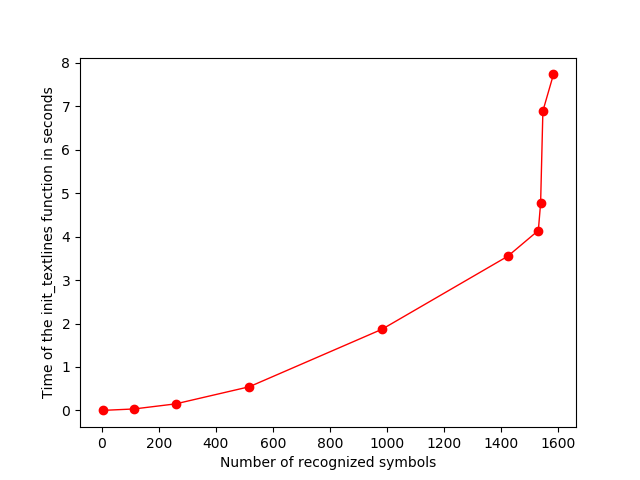
\includegraphics[height=20em]{img/results/symbolsTimeInit.png}
\caption{The dependency of the number of recognized textlines on the time of execution of the \emph{init\_textlines()} function}
\label{fig:dpiSpeed}
\end{figure}

\begin{figure}
\centering
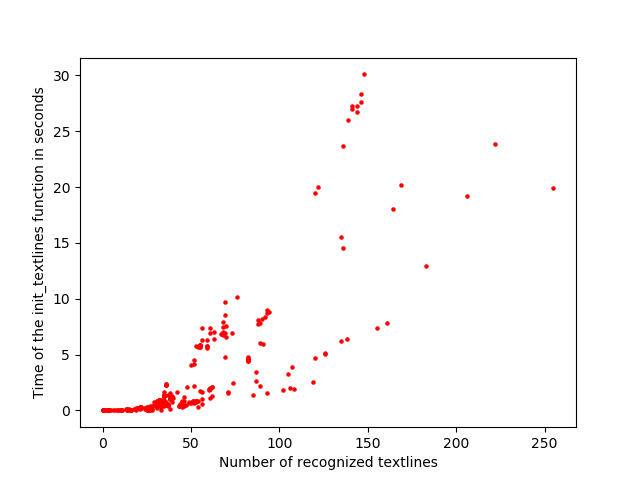
\includegraphics[height=20em]{img/results/textlinesTimeInit.png}
\caption{The dependency of the number of recognized textlines on the time of execution of the \emph{init\_textlines()} function}
\label{fig:dpiSpeed}
\end{figure}

\begin{figure}
\centering
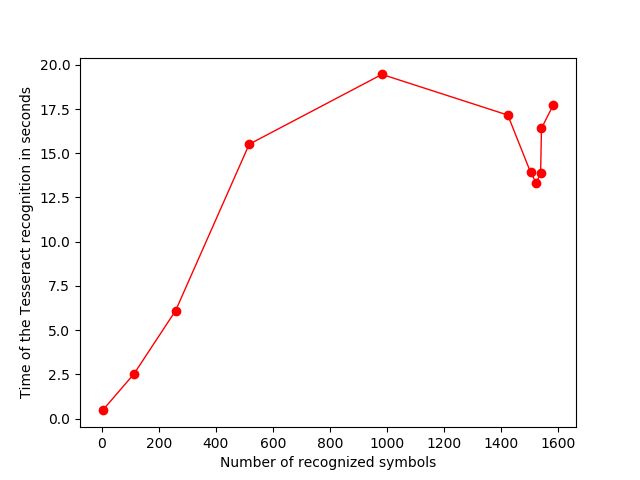
\includegraphics[height=20em]{img/results/symbolsTimeTesseract.png}
\caption{The dependency of the number of recognized textlines on the time of execution of Tesseract recognition}
\label{fig:dpiSpeed}
\end{figure}

\begin{figure}
\centering
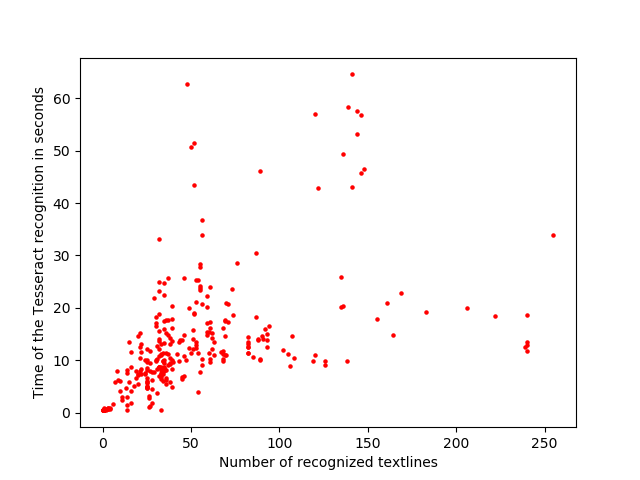
\includegraphics[height=20em]{img/results/textlinesTimeTesseract.png}
\caption{The dependency of the number of recognized textlines on the time of execution of Tesseract recognition}
\label{fig:dpiSpeed}
\end{figure}

\begin{figure}
\centering
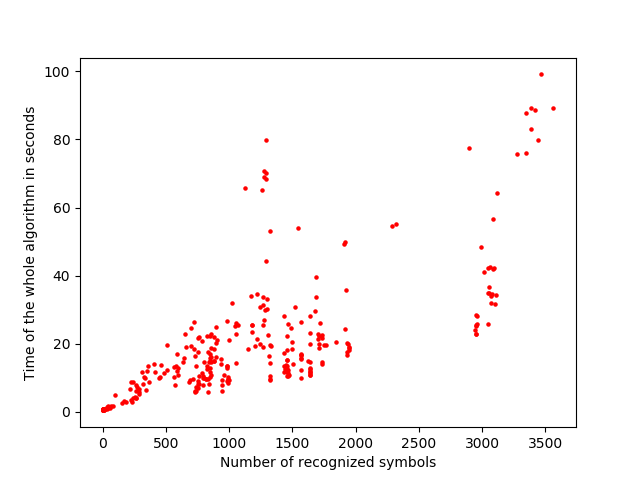
\includegraphics[height=20em]{img/results/symbolsTimeAll.png}
\caption{The dependency of the number of recognized symbols on the overall time of execution}
\label{fig:dpiSpeed}
\end{figure}

\begin{figure}
\centering
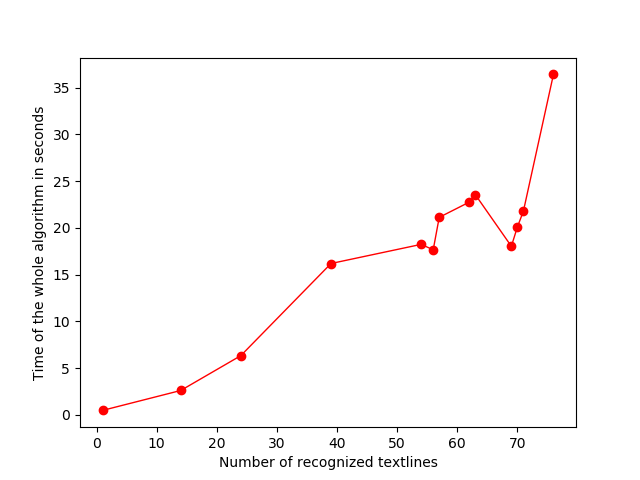
\includegraphics[height=20em]{img/results/textlinesTimeAll.png}
\caption{The dependency of the number of recognized textlines on the overall time of execution}
\label{fig:dpiSpeed}
\end{figure}

\section{Effects of image resolution}

The quality of the input image greatly affects Tesseract's recognition system and therefore our recognition system. Tesseract advises its users to use at least 300 dpi images, as it claims that lower resolution images are more likely to fail at recognition to a greater extent. In this section, we tested the effects of image resolution on both the speed of the algorithm and the accuracy of Tesseract (by which we understand the number of recognized symbols and textlines, as Tesseract outputs barely any false positives). For these purposes, we used the same different resolution images as in \xxx{tagnut hore sekciu}. We present the results in \xxx{tagnut grafy}. From the observation of the results, it is evident that the DPI of the image does not have a direct effect on the \emph{init\_textlines} function. This is because the time complexity of this function is directly dependent on the number of symbols and textlines. As a higher DPI image does not necessarily mean that more symbols and textlines will be present in the image (due to false positives, incorrect splits between textlines in lower resolution images, splitting of characters and more), the dependencies in graph \xxx{tagni} could greatly vary. However, when it comes to Tesseract recognition, we can clearly see \xxx{tag} that its execution time increases with increased DPI. What is interesting, however, is that the best execution time is achieved when the image has around 300 DPI. Although the recognition time is exponentially lower with the DPI under 150, the results from images with this resolution are of useless, as they produce many undetected characters. This might be also the reason why Tesseract advises its users to use the DPI of around 300 --- similarly to ABBYY \xxx{tag}, it might be trained to working with 300 dpi images and therefore it might always scale to this value.

This implies that the overall time complexity of our algorithm will also be dependent on the DPI of the image, with the best results obtained at the DPI of around 300.

\begin{figure}
\centering
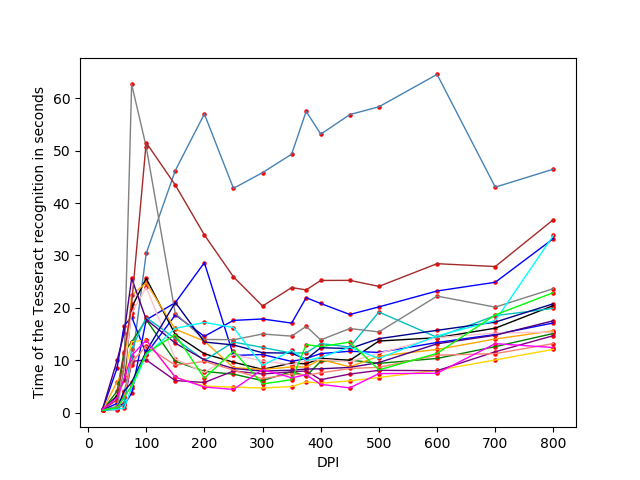
\includegraphics[height=20em]{img/results/dpiTimeTesseract.png}
\caption{The dependency of the DPI of the given image on the time of Tesseract recognition}
\label{fig:dpiSpeed}
\end{figure}

\begin{figure}
\centering
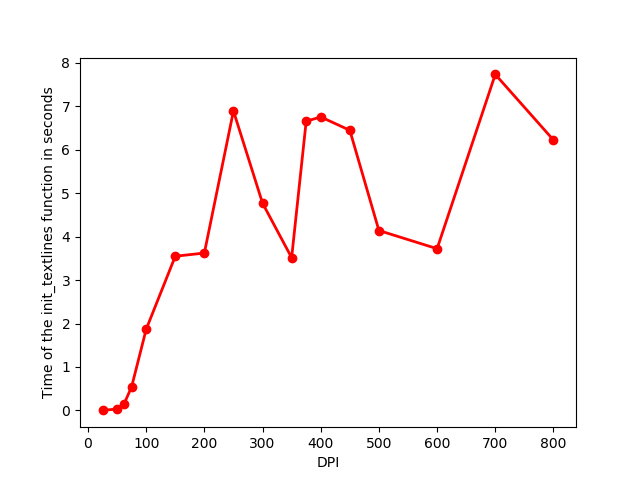
\includegraphics[height=20em]{img/results/dpiTimeInit.png}
\caption{The dependency of the DPI of the given image on the \emph{init\_textlines} function}
\label{fig:dpiSpeed}
\end{figure}

\begin{figure}
\centering
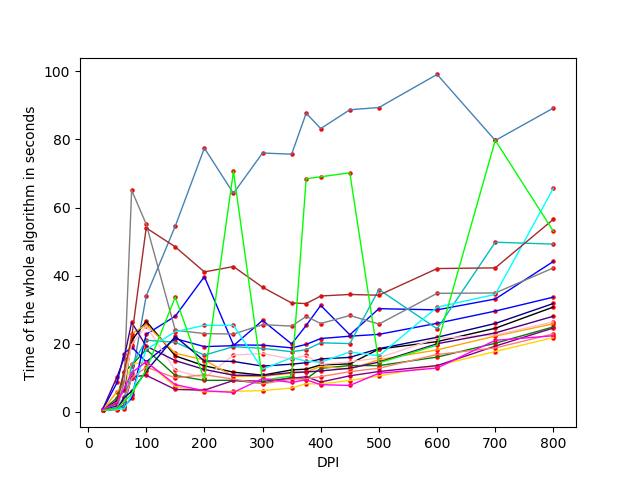
\includegraphics[height=20em]{img/results/dpiTimeAll.png}
\caption{The dependency of the DPI of the given image on the overall time of our algorithm}
\label{fig:dpiSpeed}
\end{figure}

\section{Effects of preprocessing}

As mentioned multiple times in the previous chapters, preprocessing is a crucial part of any OCR engine, including Tesseract. In \xxx{taggni figure}, we will show its importance along with a few examples of how the recognition results change when only slight tweaks in an image are made.

\begin{figure}[t]
\centering

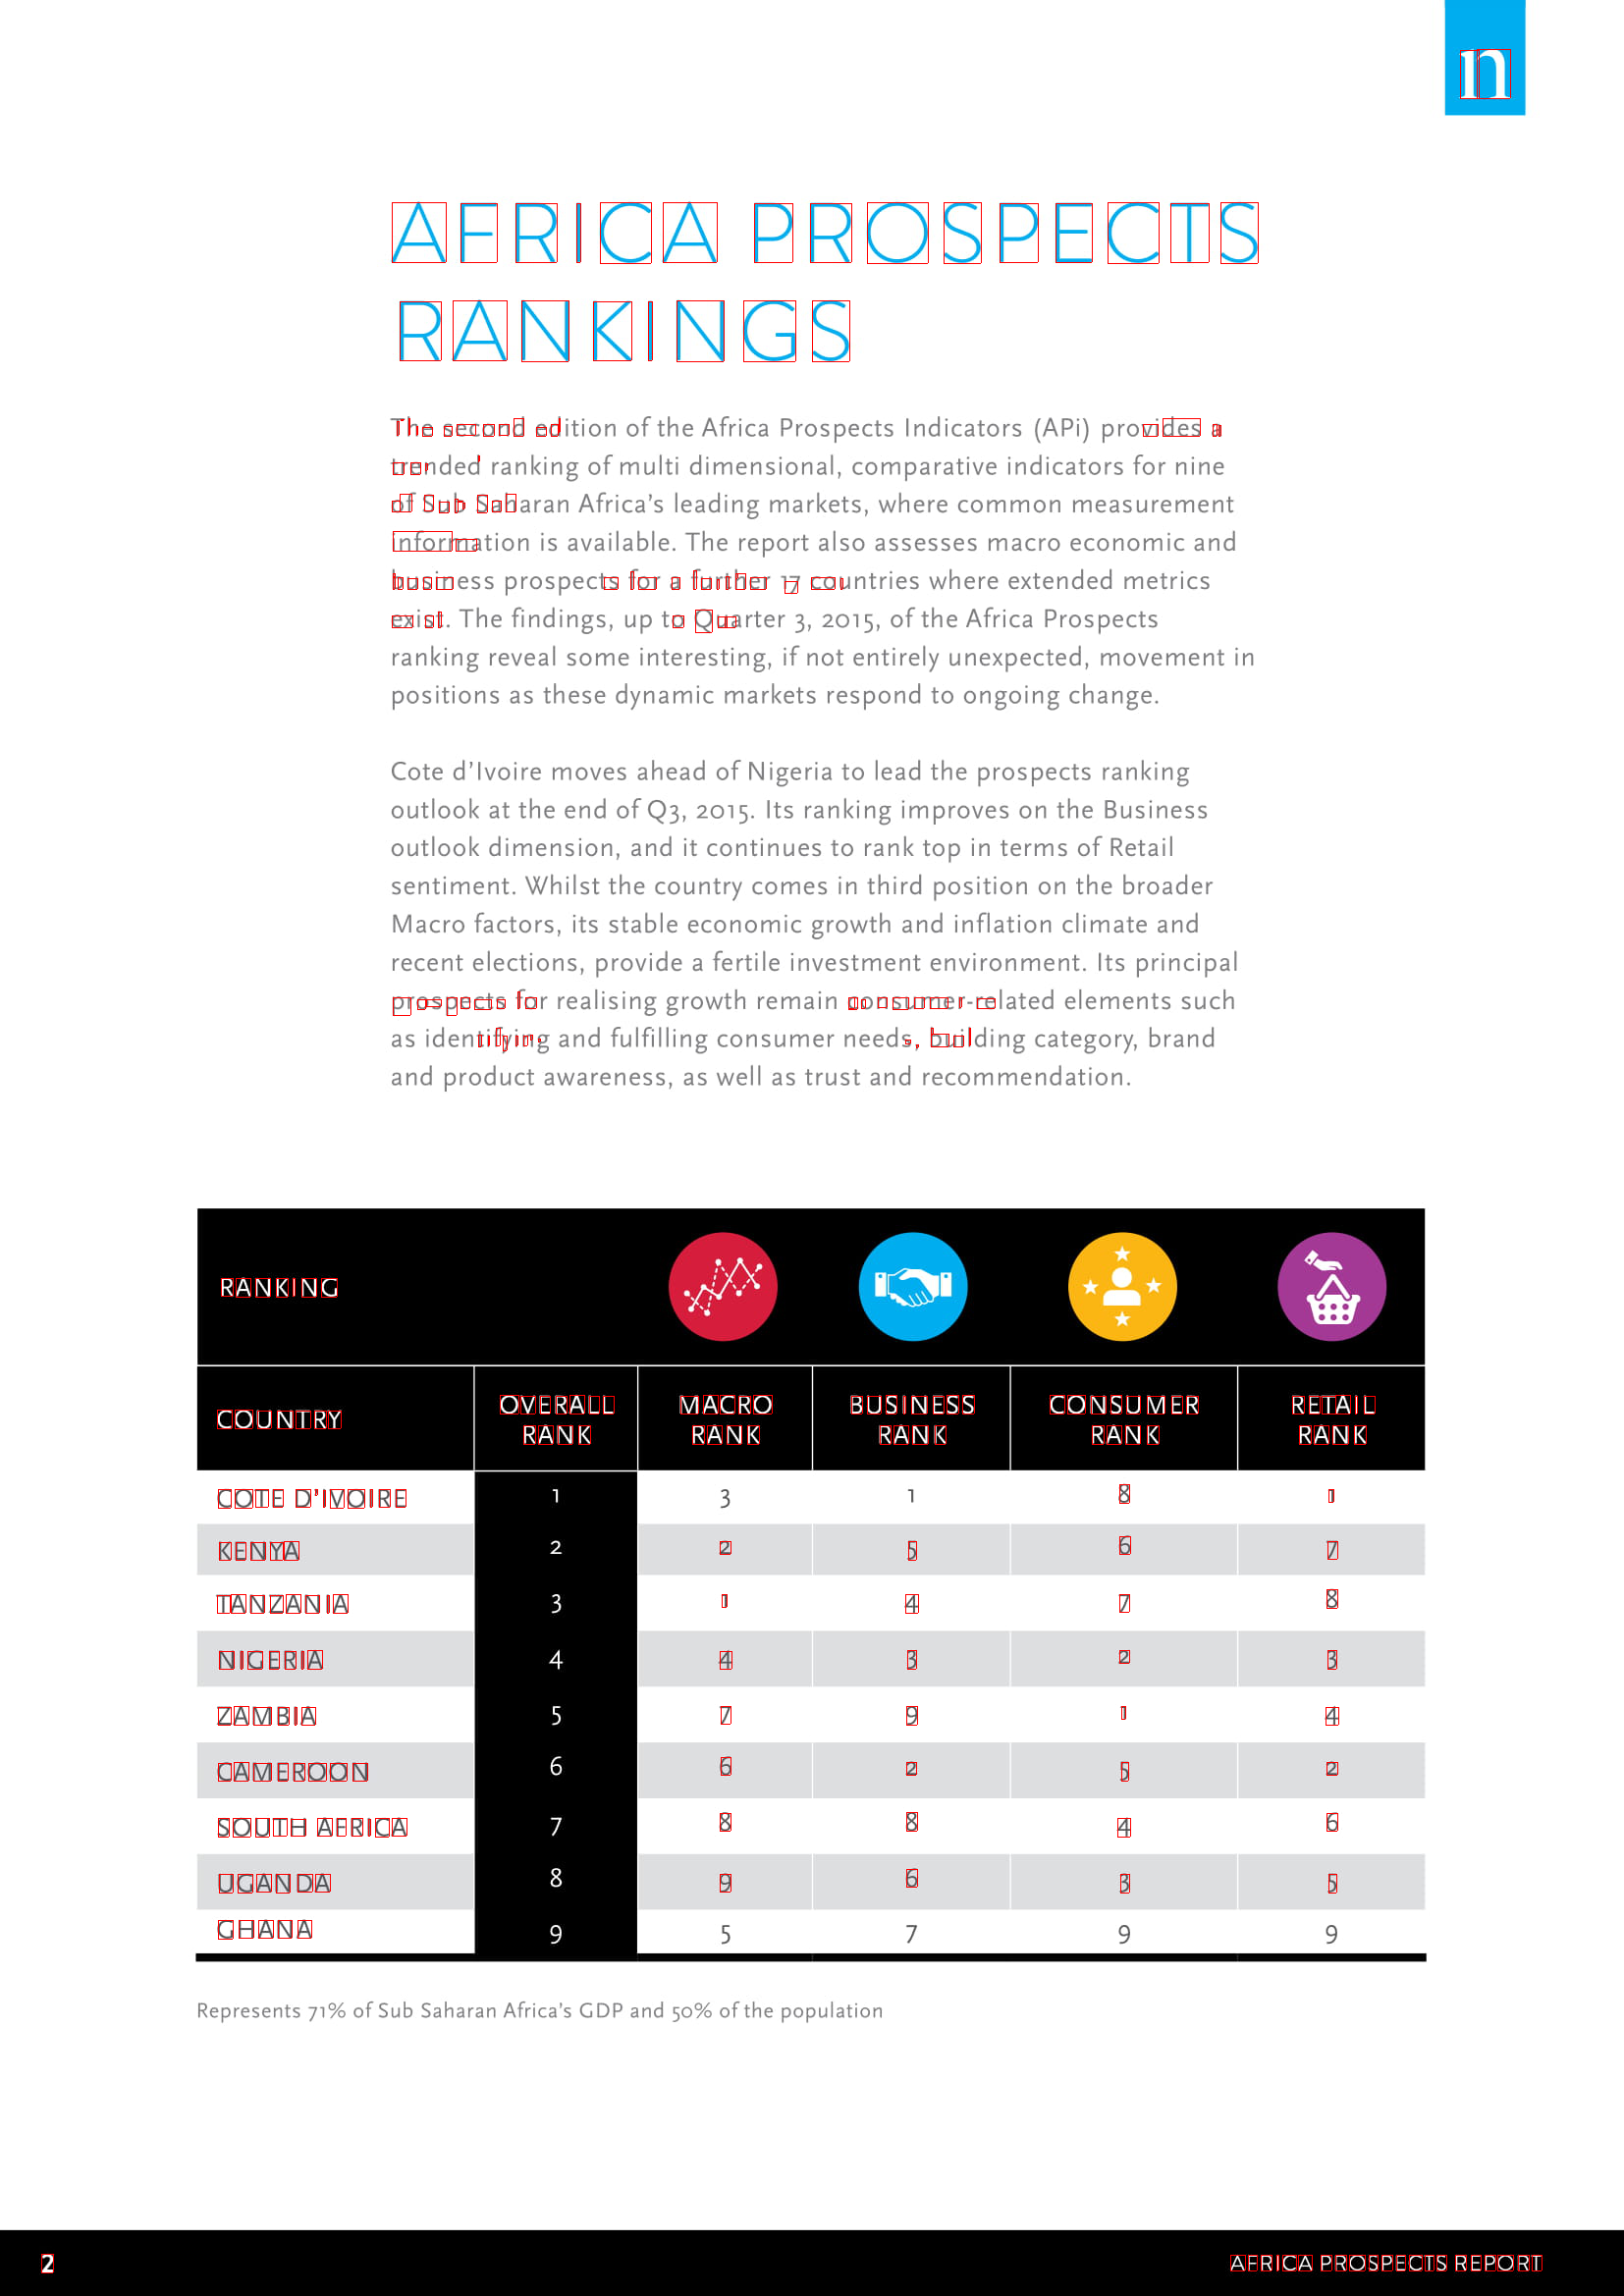
\includegraphics[width=15em]{img/results/im1_noPreproc.png}
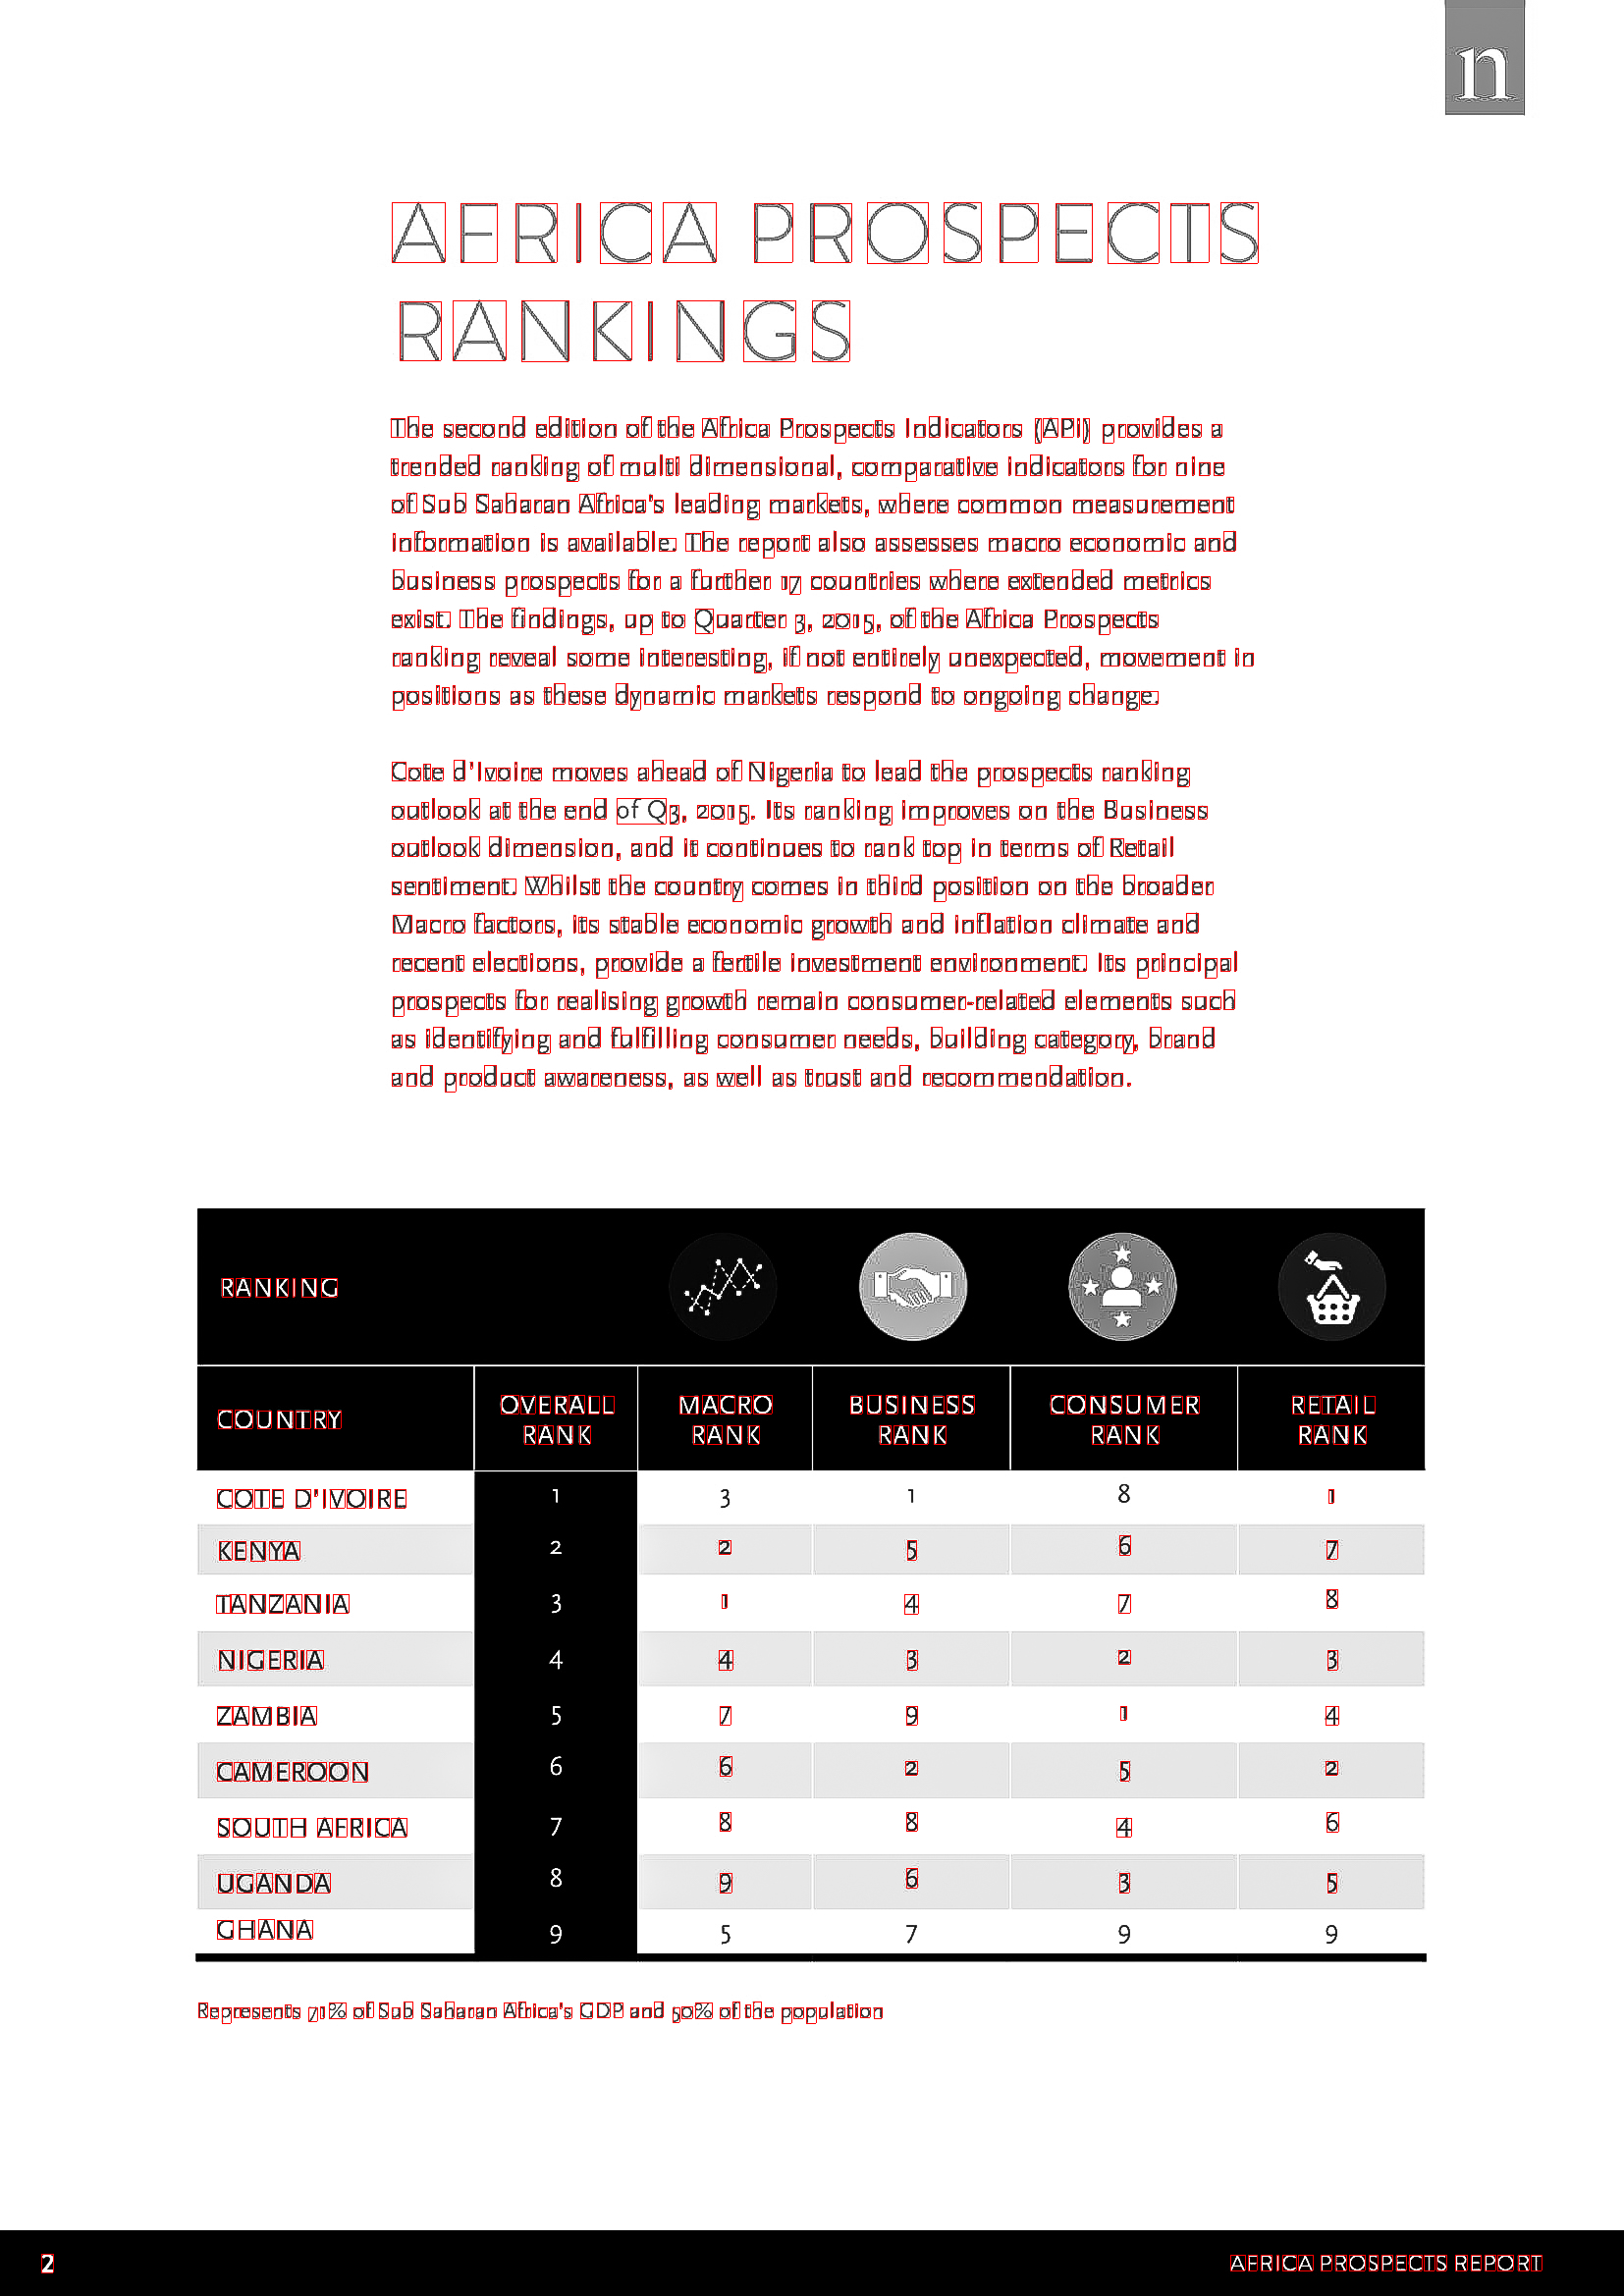
\includegraphics[width=15em]{img/results/im1_Preproc.png}

\caption{The effects of preprocessing on Tesseract recognition. Left: Tesseract does recognize most of the symbols of the original image because of low contrast. Right: Upon applying a simple luma greyscale conversion and increasing contrast, Tesseract renders notably better results.}
\label{fig:preprocessEffects}
\end{figure}

\begin{figure}[t]
\centering

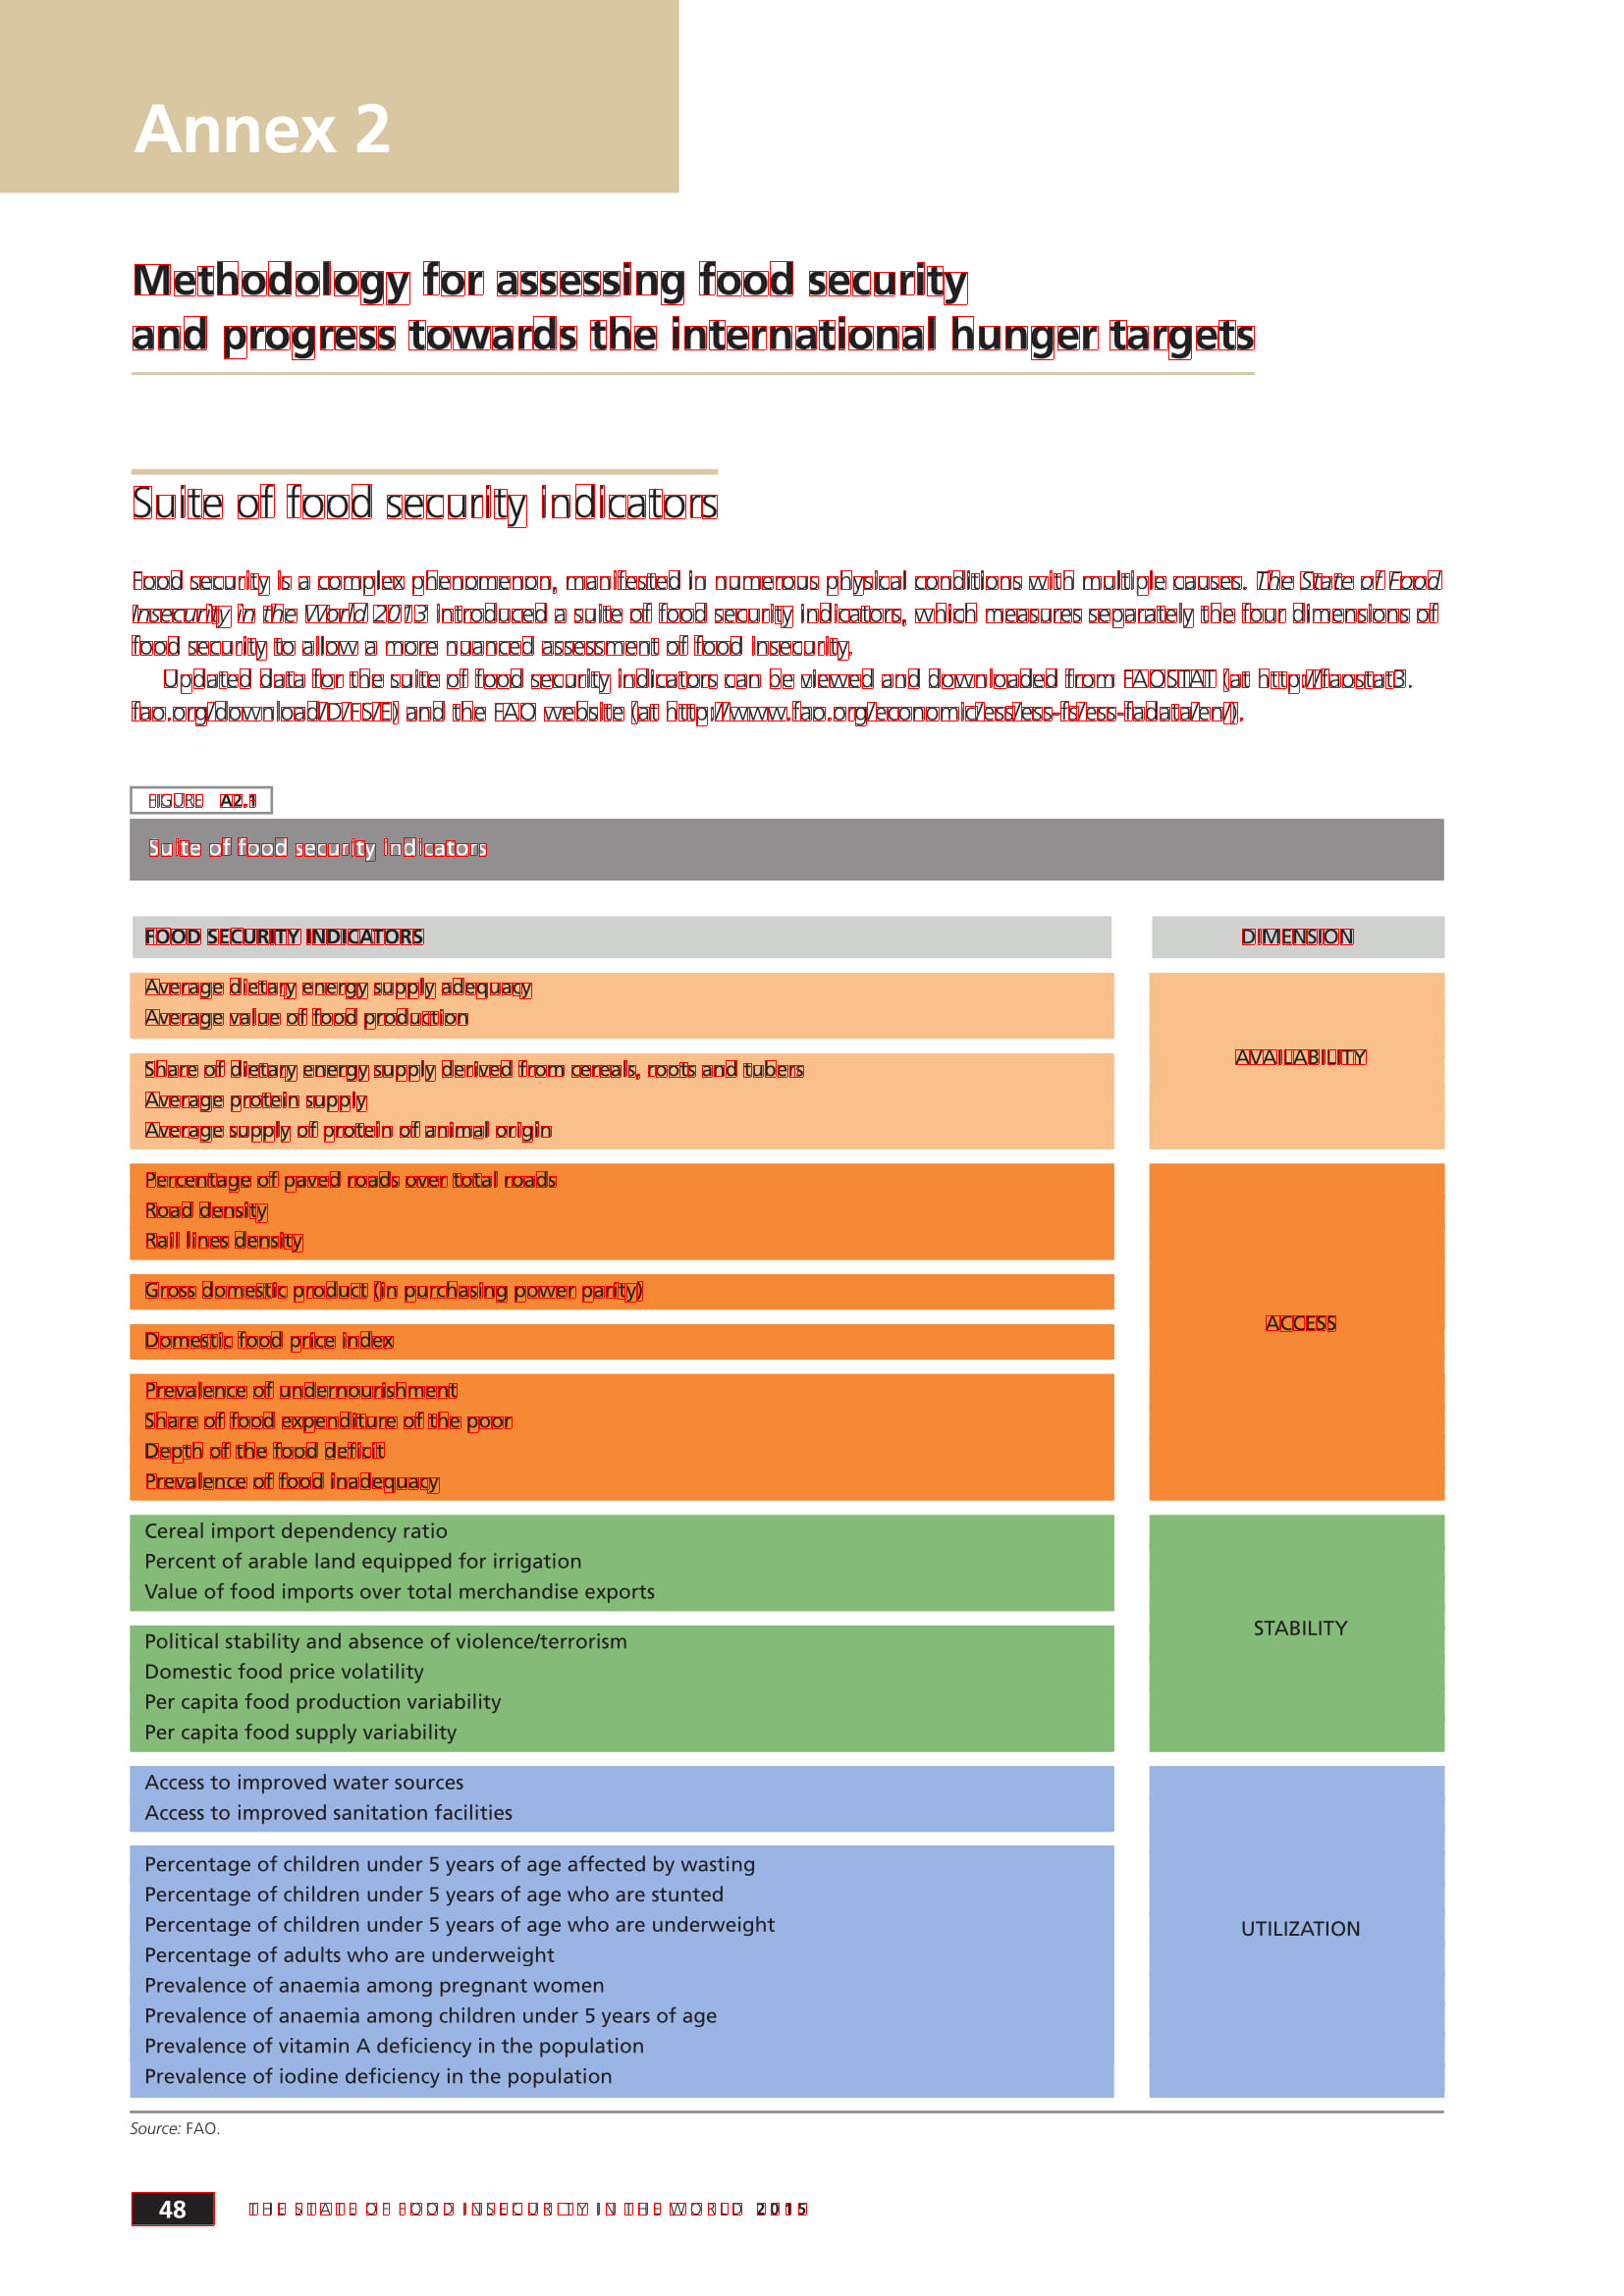
\includegraphics[width=16em]{img/results/im2_noPreproc.png}
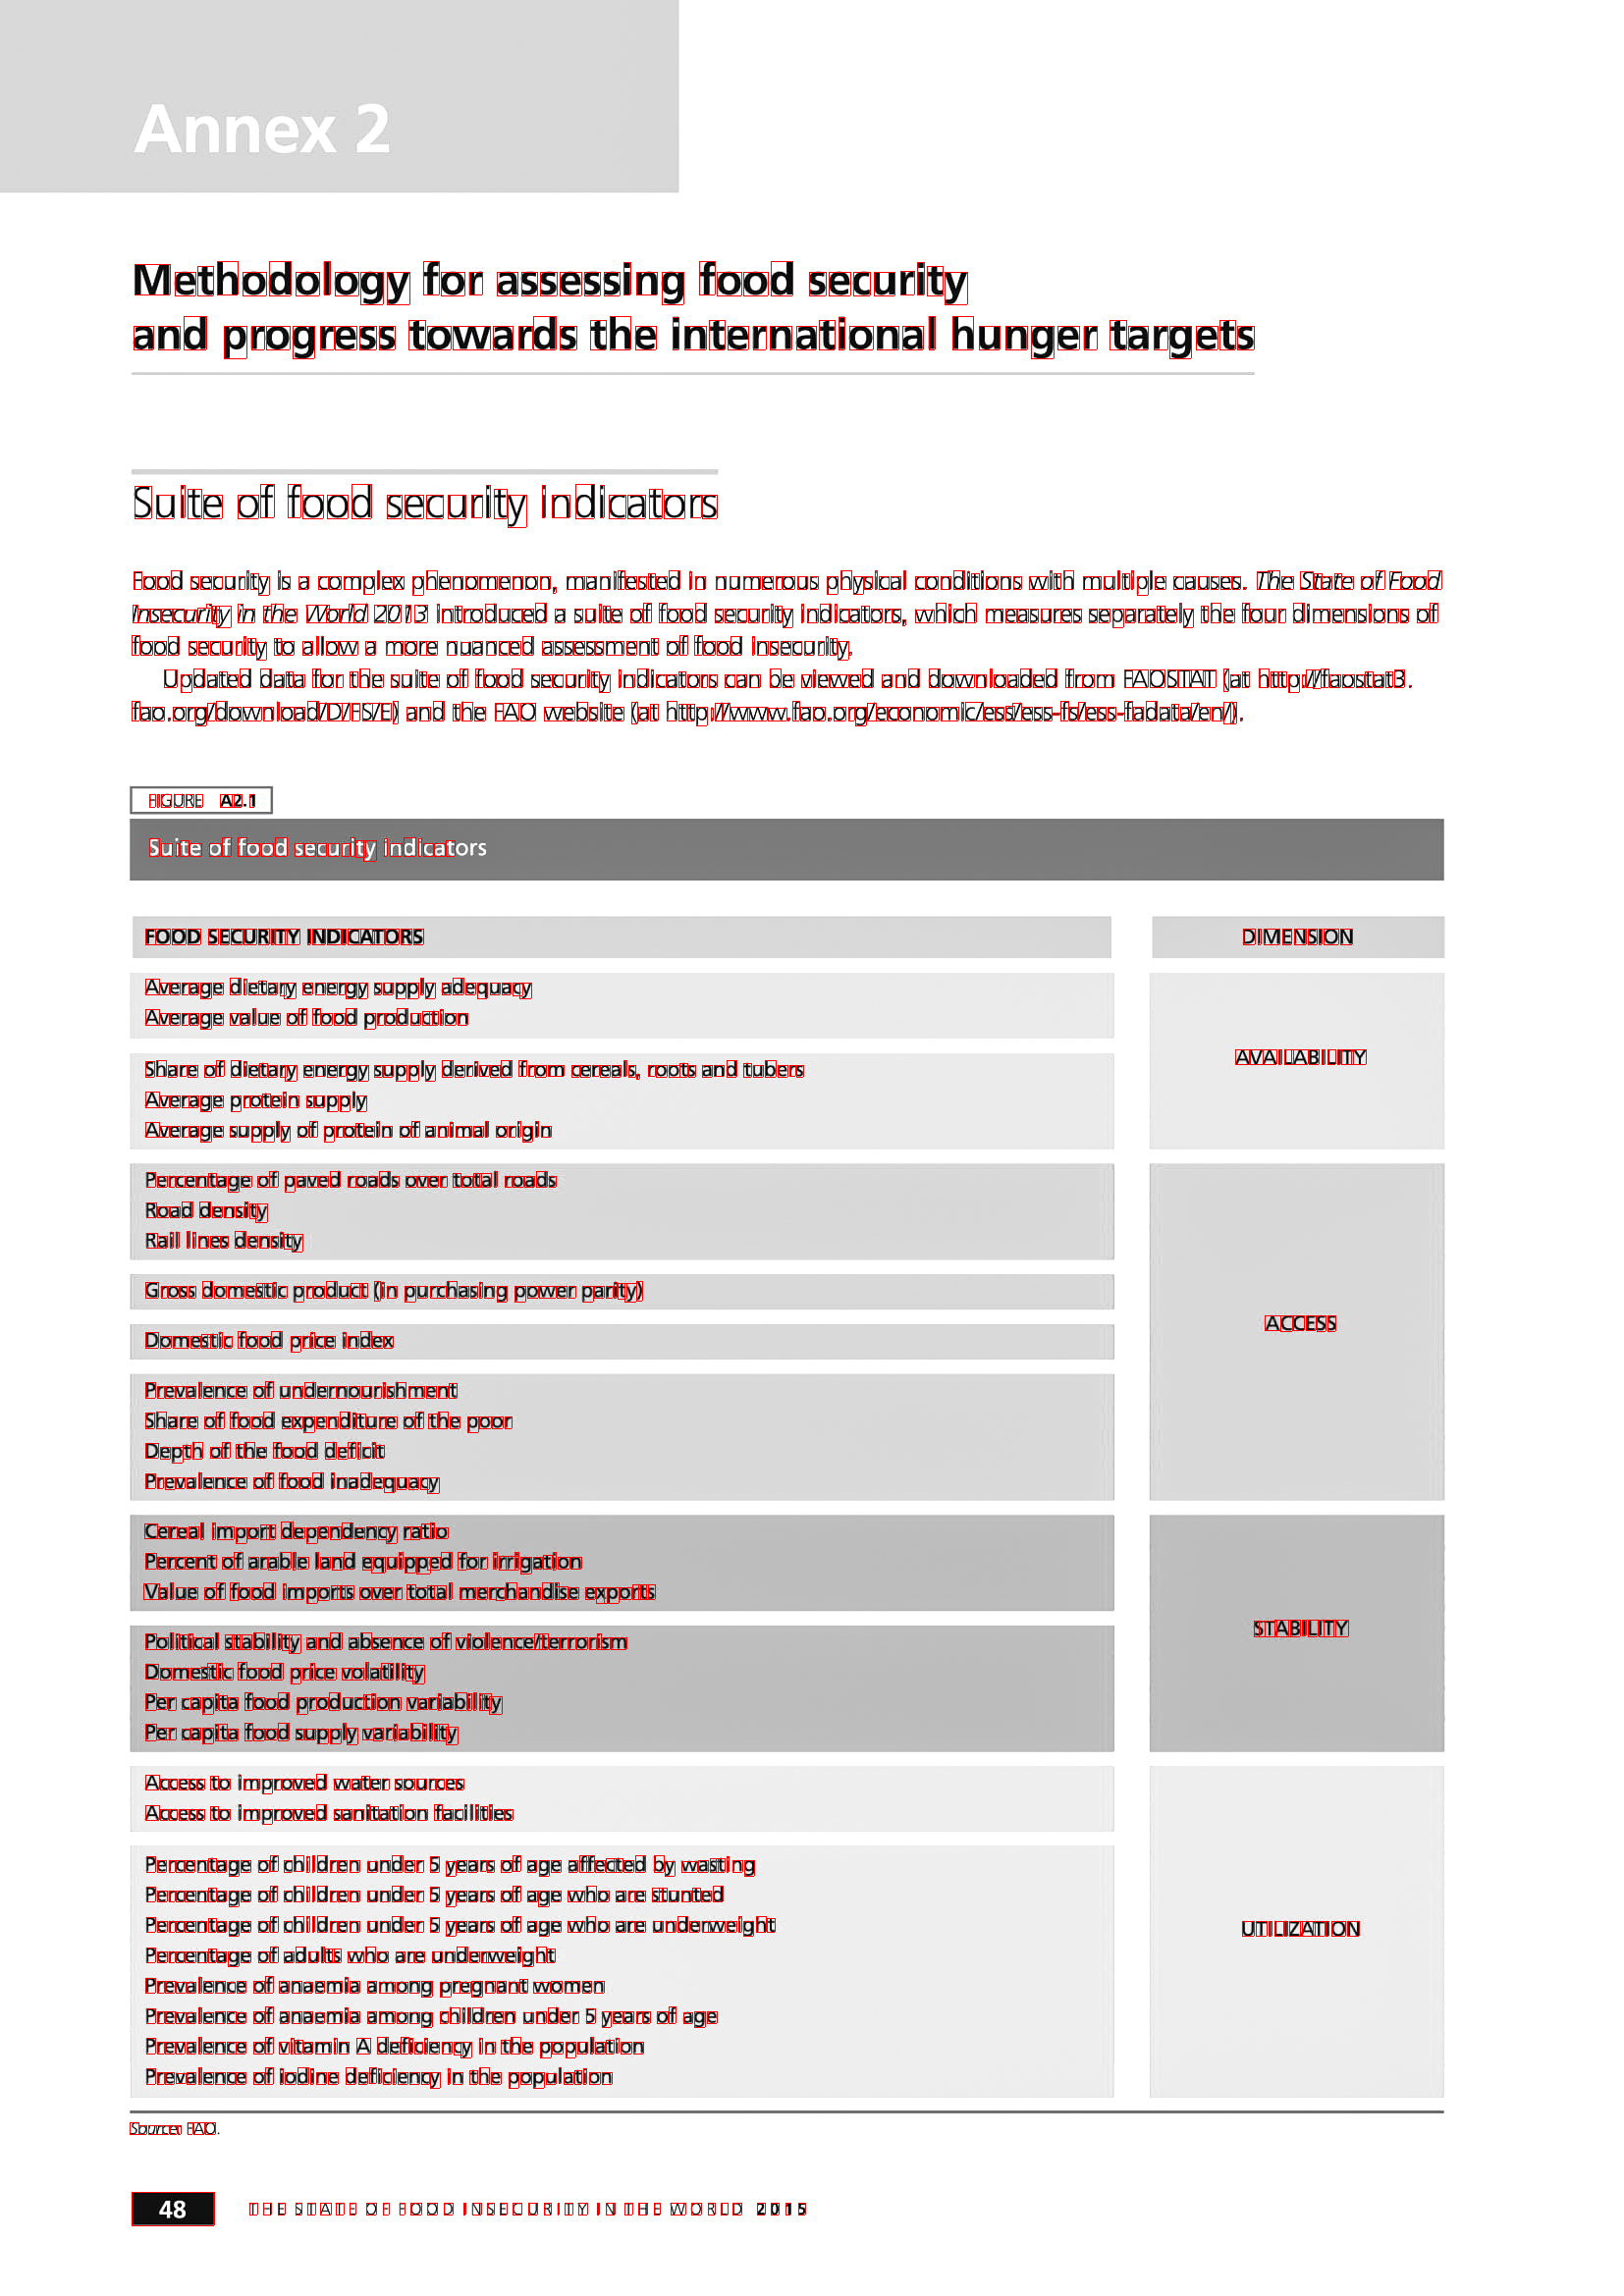
\includegraphics[width=16em]{img/results/im2_Preproc.png}

\caption{The effects of preprocessing on Tesseract recognition. Left: The lower part of the image is not recognzied properly due to a dark background. Right: Tesseract recognizes all the symbols of the image once it is preprocessed by applying an adaptive greyscale conversion (by lowering blues, reds, yellows and greens).}
\label{fig:preprocessEffects}
\end{figure}

\section{Comparison to Tesseract's tablefind}

We already mentioned Tesseract's tablefind algorithm in \xxx{tagnut}. It uses heuristical algorithms to find tables from the segmentation Tesseract already offers. It also contains a simple recognition class that tries to analyze the found table for rows, columns and cells. It is a bottom-down approach, in comparison to our algorithm, which starts from the individual characters and builds up a table.

Although this algorithm has a pretty impressive results when finding tables (\emph{table detection}), it does not provide any information about the text in various cells and has no output except for a bounding box around the found table. Therefore, there is almost no support for table recognition, which was the goal our implementation was focused on.

Moreover, tablefind is not user-friendly and is mainly used as a tool for developers. It has no command line interface and GUI and the user needs to understand its API to obtain its results.

Although, in a lot of cases, its table detection renders better results than ours, the results are overall incomparable, as the goals of tablefind and our system are different.

\section{Our results}

In \xxx{figure}, we provide a few sample results of our algorithm. Following are the most visible problems that our algorithm encounters, along with an outline of their solutions:

\begin{itemize}
    \item \emph{Tables bordered by horizontal and vertical lines}
    
    Presented in \xxx{fig}, this most basic example of a table is something we completely ignore in our algorithm. Once we assume that a textline recognized by Tesseract is either a simple horizontal or vertical line, or even a border around a segmentation element, we automatically remove it as it may disrupt with our recognition process.
    
    Rather than ignoring these lines, we could first implement a heuristical algorithm trying to combine these lines together and determine whether they might not be presenting a table.
    
    \item \emph{Word whitespace detection}
    
    Although column detection seems to work quite well, word whitespace detection has great room for improvement. Presented in \xxx{fig}, more often than not, the estimated whitespace is greater than the real value, which results in merging words that should be separated. As already mentioned in \xxx{tag implemen}, the approach with various font categories had better results with the estimation of whitespaces. We replaced this approach by the current because of the complications that arose when calculating column whitespace. Also, this approach would increase the time complexity of the algorithm, as it contained a number of other iterations of symbols and textlines. However, to increase the accuracy of word whitespace detection, the better practice would be to use the old approach for word whitespace detection, and the new for column whitespace detection. 
    
    \item \emph{Multi-row columns}
    
    As we can see in \xxx{figure}, the detection of multi-rows does not work very effectively. This is because of our constant based algorithm. We could try to improve this by implementing of a smarter algorithm based on heuristics. For example. one of the possible implementation could try to get all of the gaps between lines in a table a determine the spaces similarly to our whitespace detection. Also, when every third cell's text starts with an upper case letter, and all the others start with a lower case, it is a pretty clear indicator of the presence of a multi-row cell.
    
    \item \emph{Multi-column layouts}
    
    Our algorithm has no support for multi-column layouts. This results in either merging tables from different columns into one, or recognizing each table from different columns as a single column table, as the whitespace between columns can be quite big compared to other whitespaces. This can be solved by firstly checking whether the page is multi-column (by finding wide whole-page columns that contain no symbols), and then applying our algorithm to each of the recognized columns.
    
    \item \emph{Different languages support}
    
    Right now, we initialize Tesseract with a testing data suitable for character of the English language. Tesseract still recognizes symbols from other languages (like é, ô, ñ and many more), but instead of outputing the symbol we wished for, it returns a combination of non-alphabetical ASCII characters. Although this does not interfere with the image output of our table recognition, it notably affects the json output.
    
    This can be solved by adding other testing data from the Tesseract open source repository and implementing their usage.
    
    \item \emph{Support of only simple table structure}
    
    Our system does not recognize complicated table structures \xxx{tag figure}, and relies on the tables to have a simple grid layout. The structure of our algorithm has no support for handling other kinds of table structure (although our json output file could output them). Therefore, to solve this problem, a lot of serious changes needs to be made in our function that merges lines into tables, such as isolating the tables, checking for their headers, segmentation of the tables and maybe even a semantical analysis.  
    
    \item \emph{Other errors}
    
    There are multiple other errors that need to be fixed. These include unrecognized headers of tables, table splits, recognition of graphics as tables, no support for vertical text and others. We present a few of them in \xxx{fig}.
    
\end{itemize}


TO DO
word whitespace
table bordered

\begin{figure}[t]
\centering
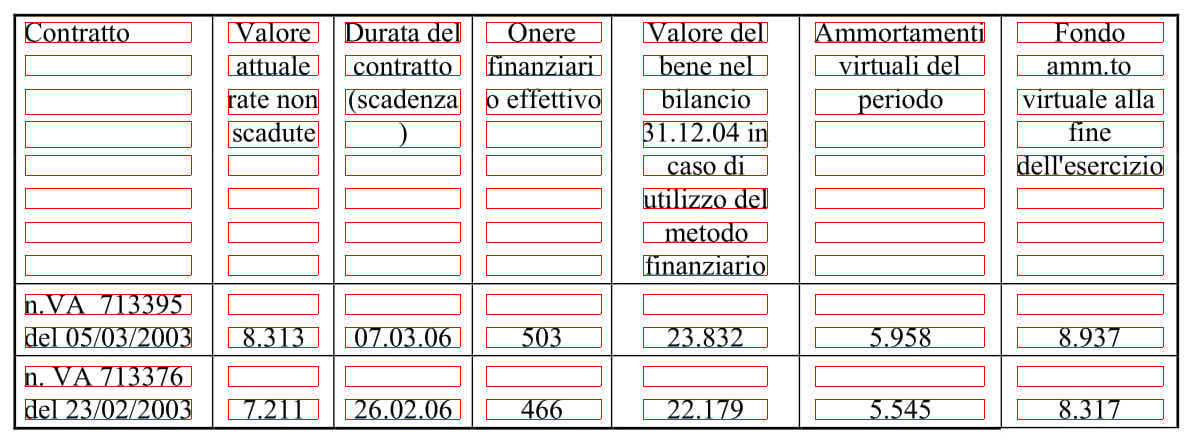
\includegraphics[width=20em]{img/results/errorMultiRow.png}
\caption{Improperly recognized multi-row cells}
\label{fig:errors}
\end{figure}

\begin{figure}[t]
\centering
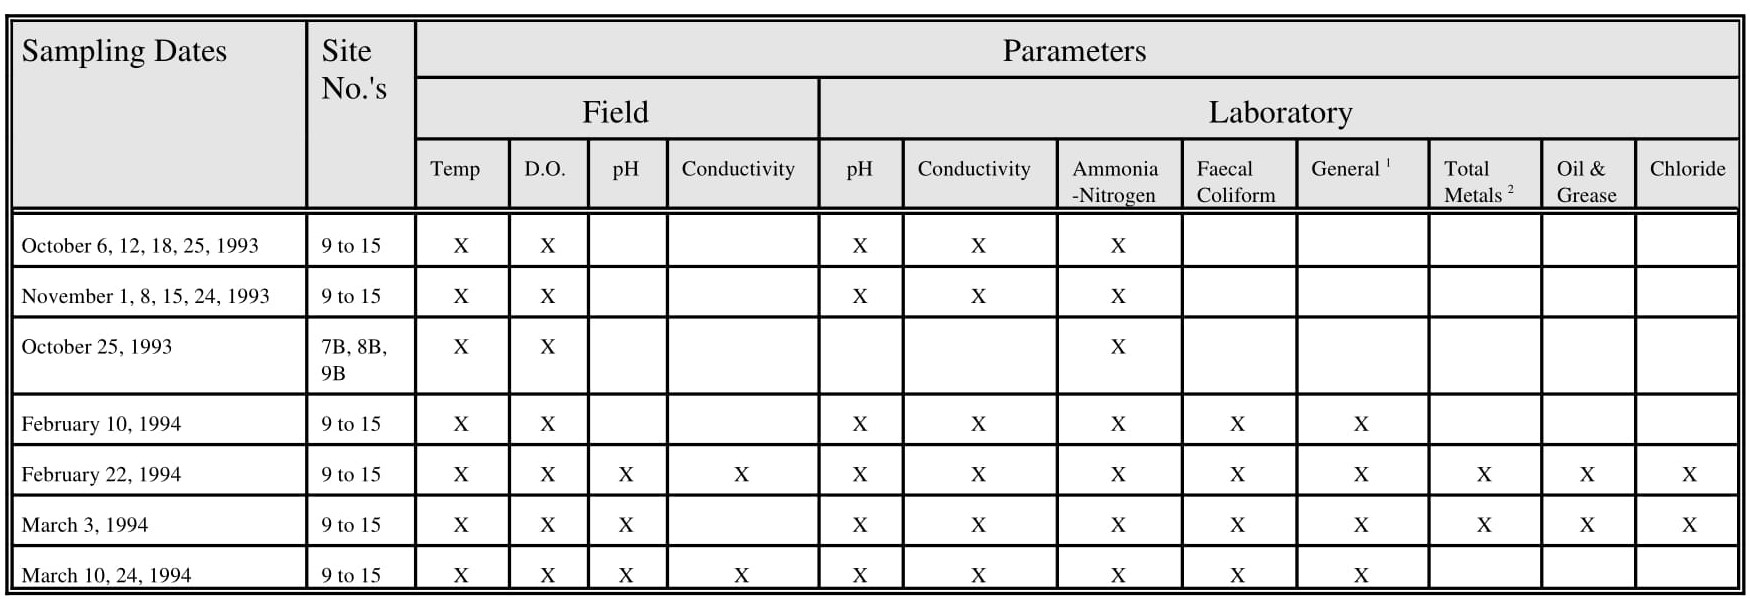
\includegraphics[width=20em]{img/results/errorStructure.jpg}
\caption{Complicated table structure}
\label{fig:errors}
\end{figure}

\begin{figure}[t]
\centering

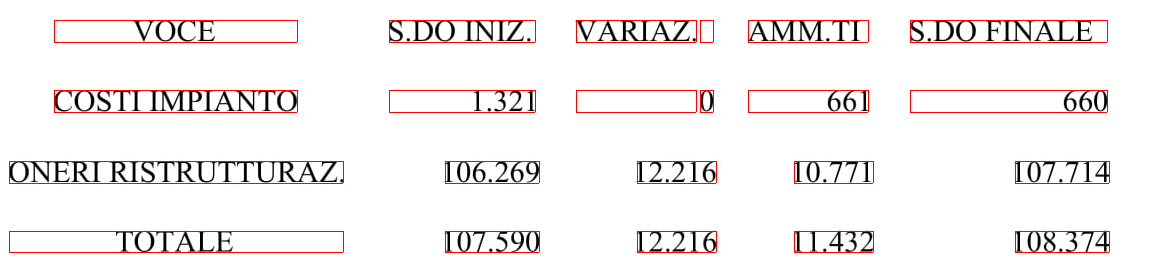
\includegraphics[width=15em]{img/results/otherErr1Cell.png}
\qquad
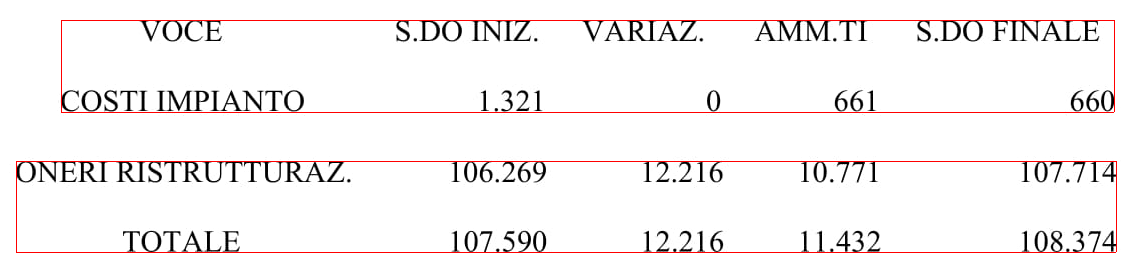
\includegraphics[width=15em]{img/results/otherErr1Table.png}

\caption{Table split errors. Although the image contains only one table, two are recognized. Our algorithm assumes that the first table has 6 columns, while the second has only 5 which do not align properly.
Left: Recognized tables by cells Right: Borders of the recognized tables}
\label{fig:errors}
\end{figure}

\begin{figure}[t]
\centering
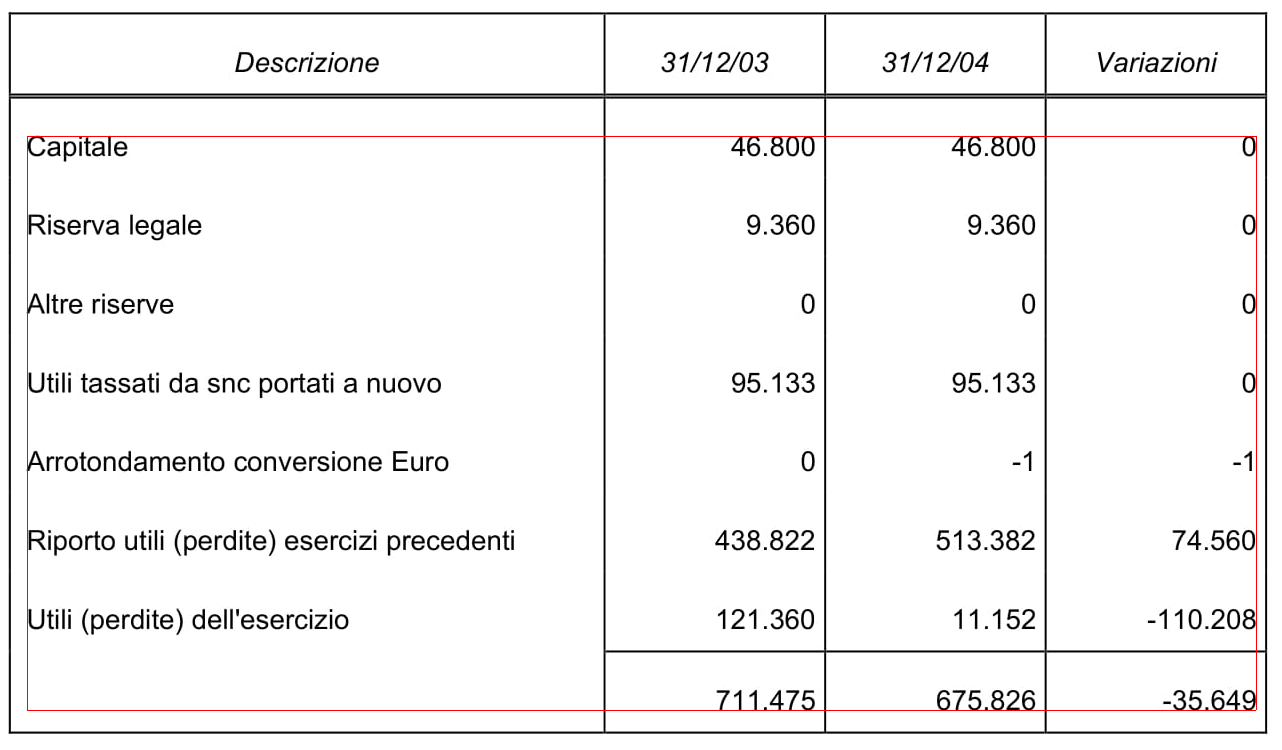
\includegraphics[width=15em]{img/results/otherErr2.png}
\caption{Unrecognized table headers}
\label{fig:errors}
\end{figure}

\begin{figure}[t]
\centering
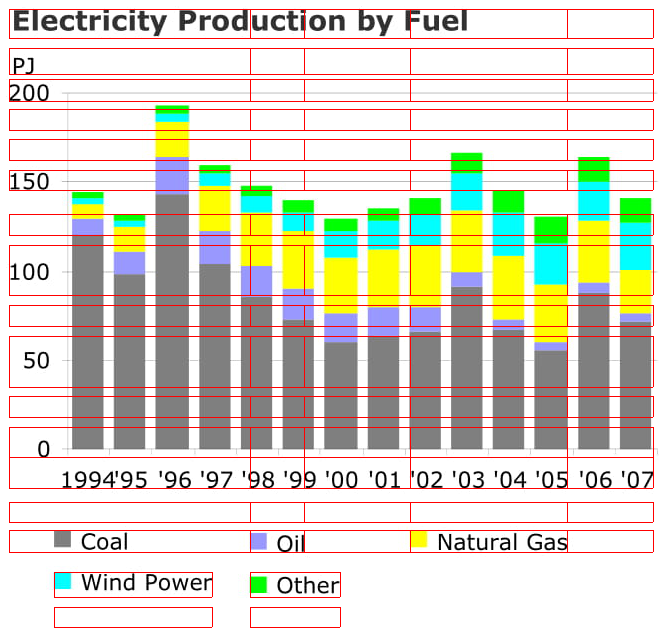
\includegraphics[width=15em]{img/results/otherErr3.png}
\caption{Our algorithm's influence on graphics images.}
\label{fig:errors}
\end{figure}

\begin{figure}[t]
\centering
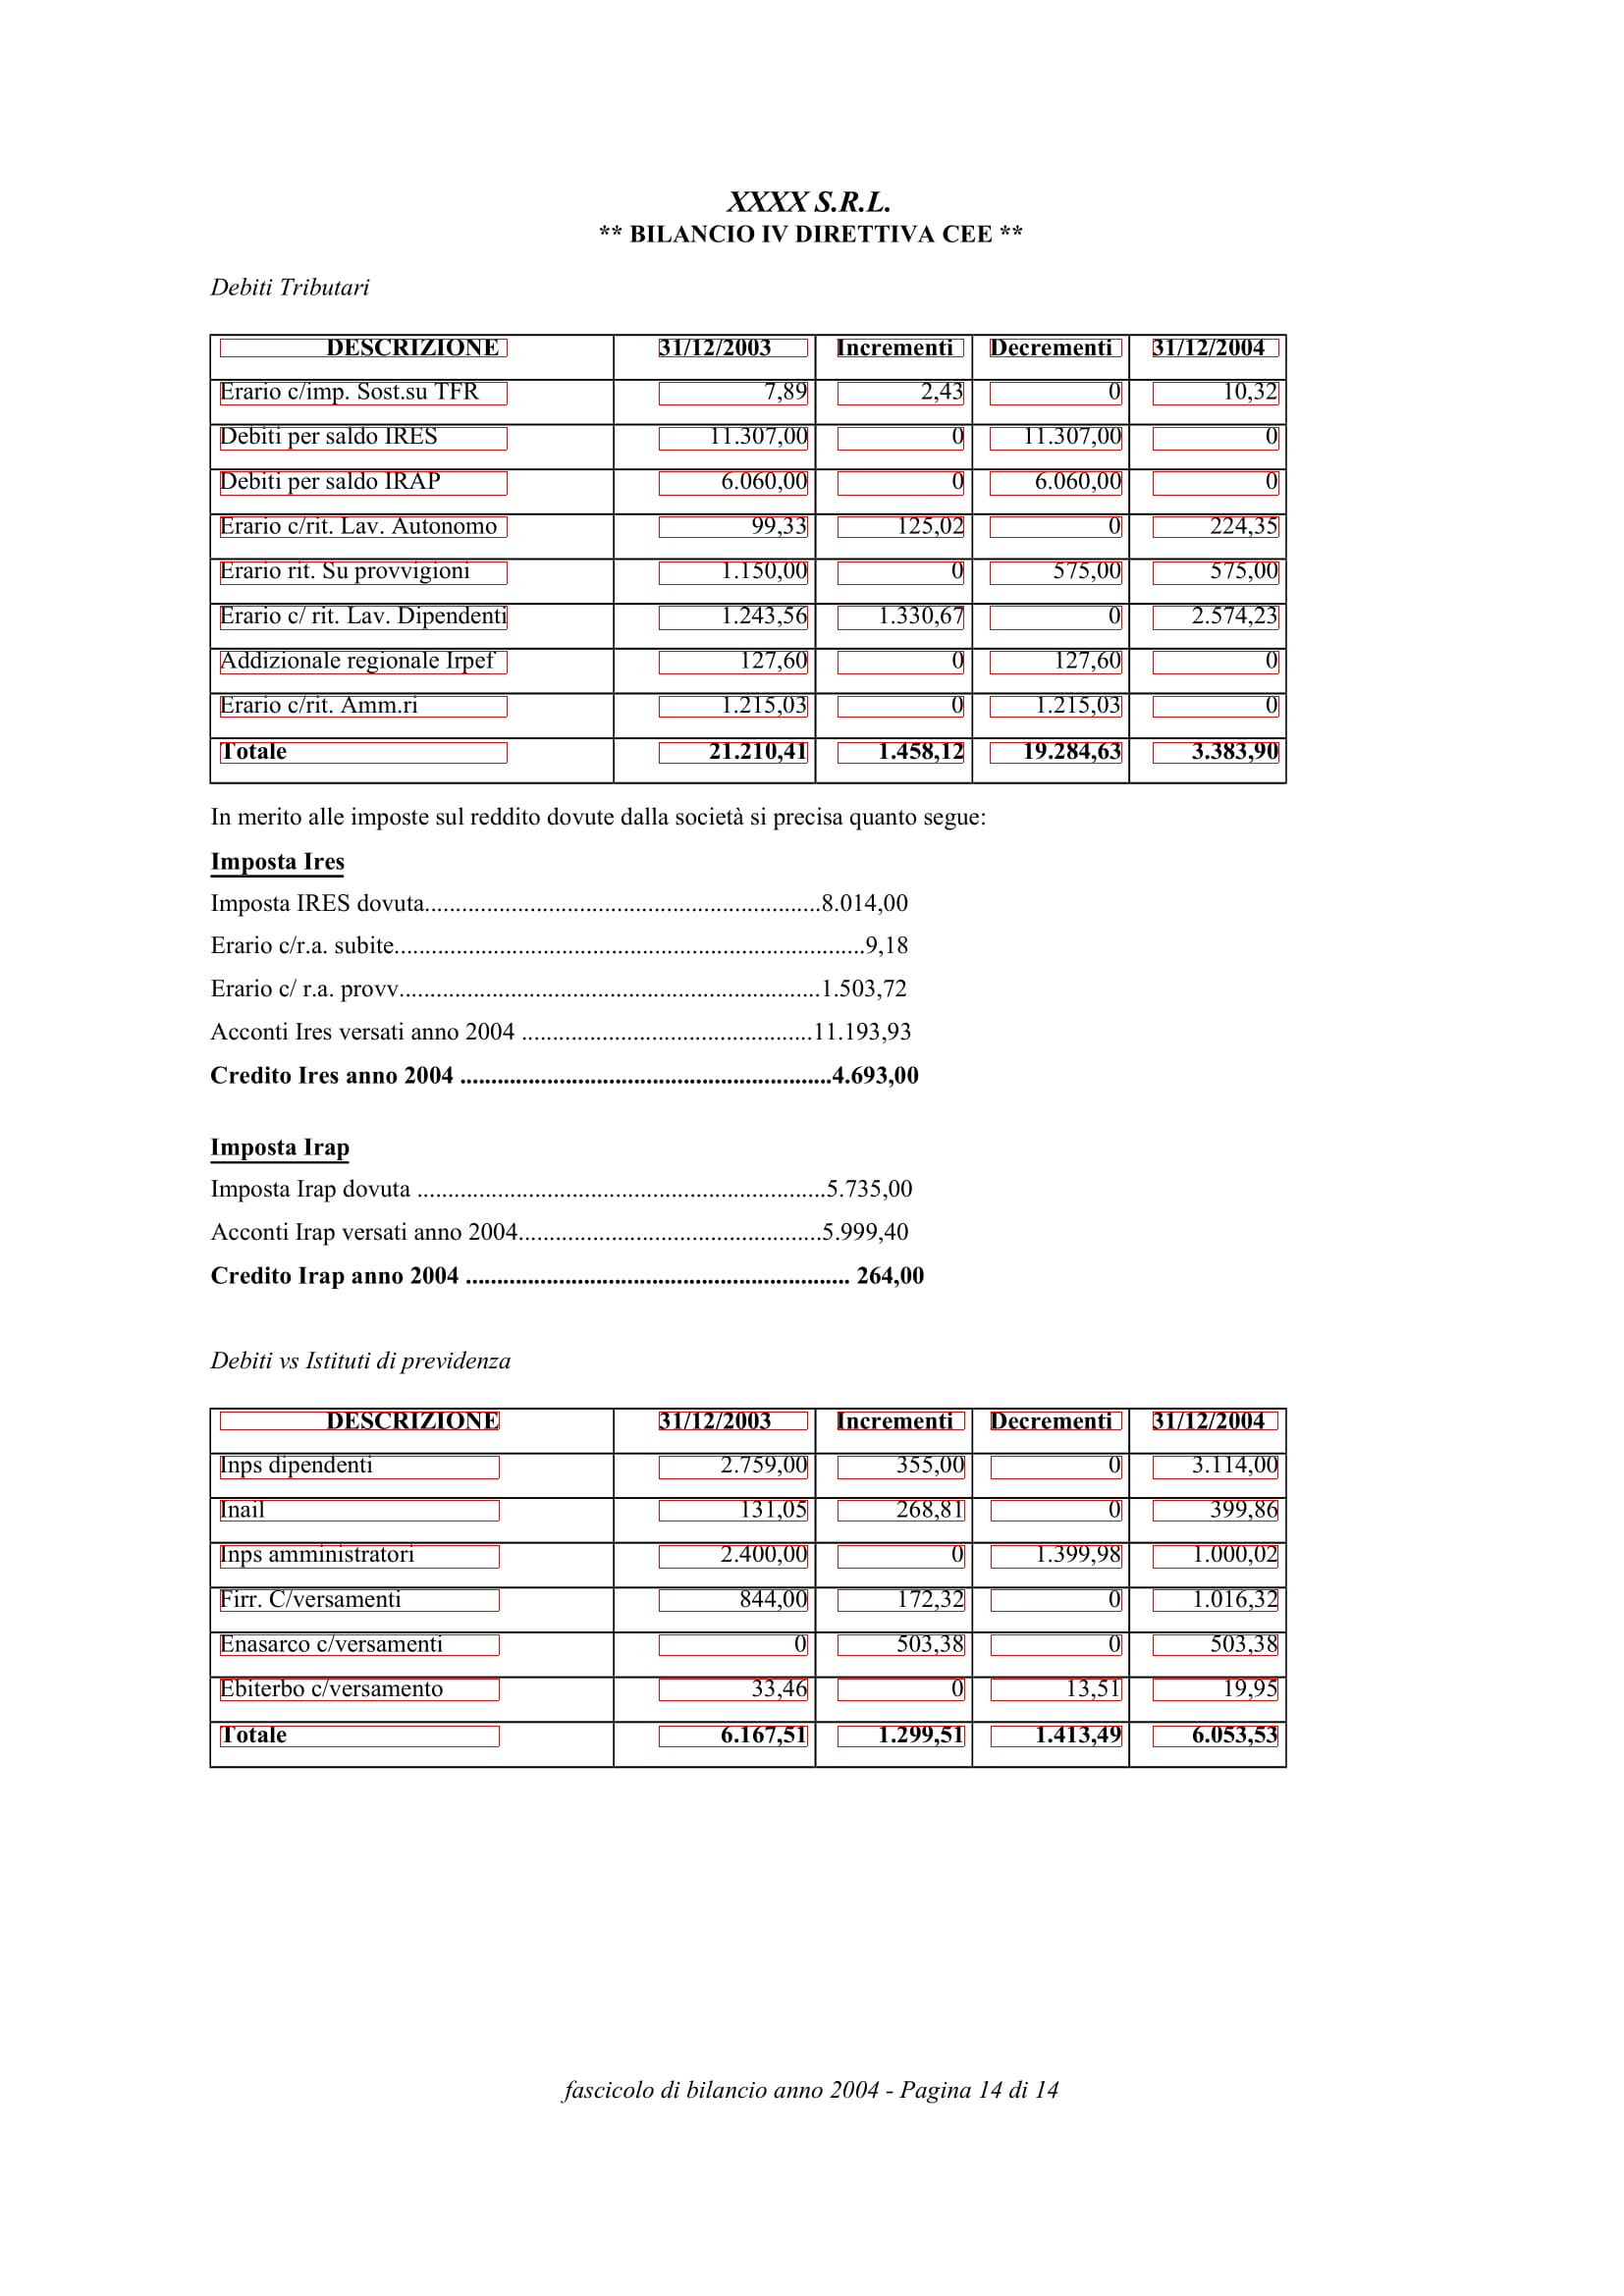
\includegraphics[width=15em]{img/results/goodRes1.png}
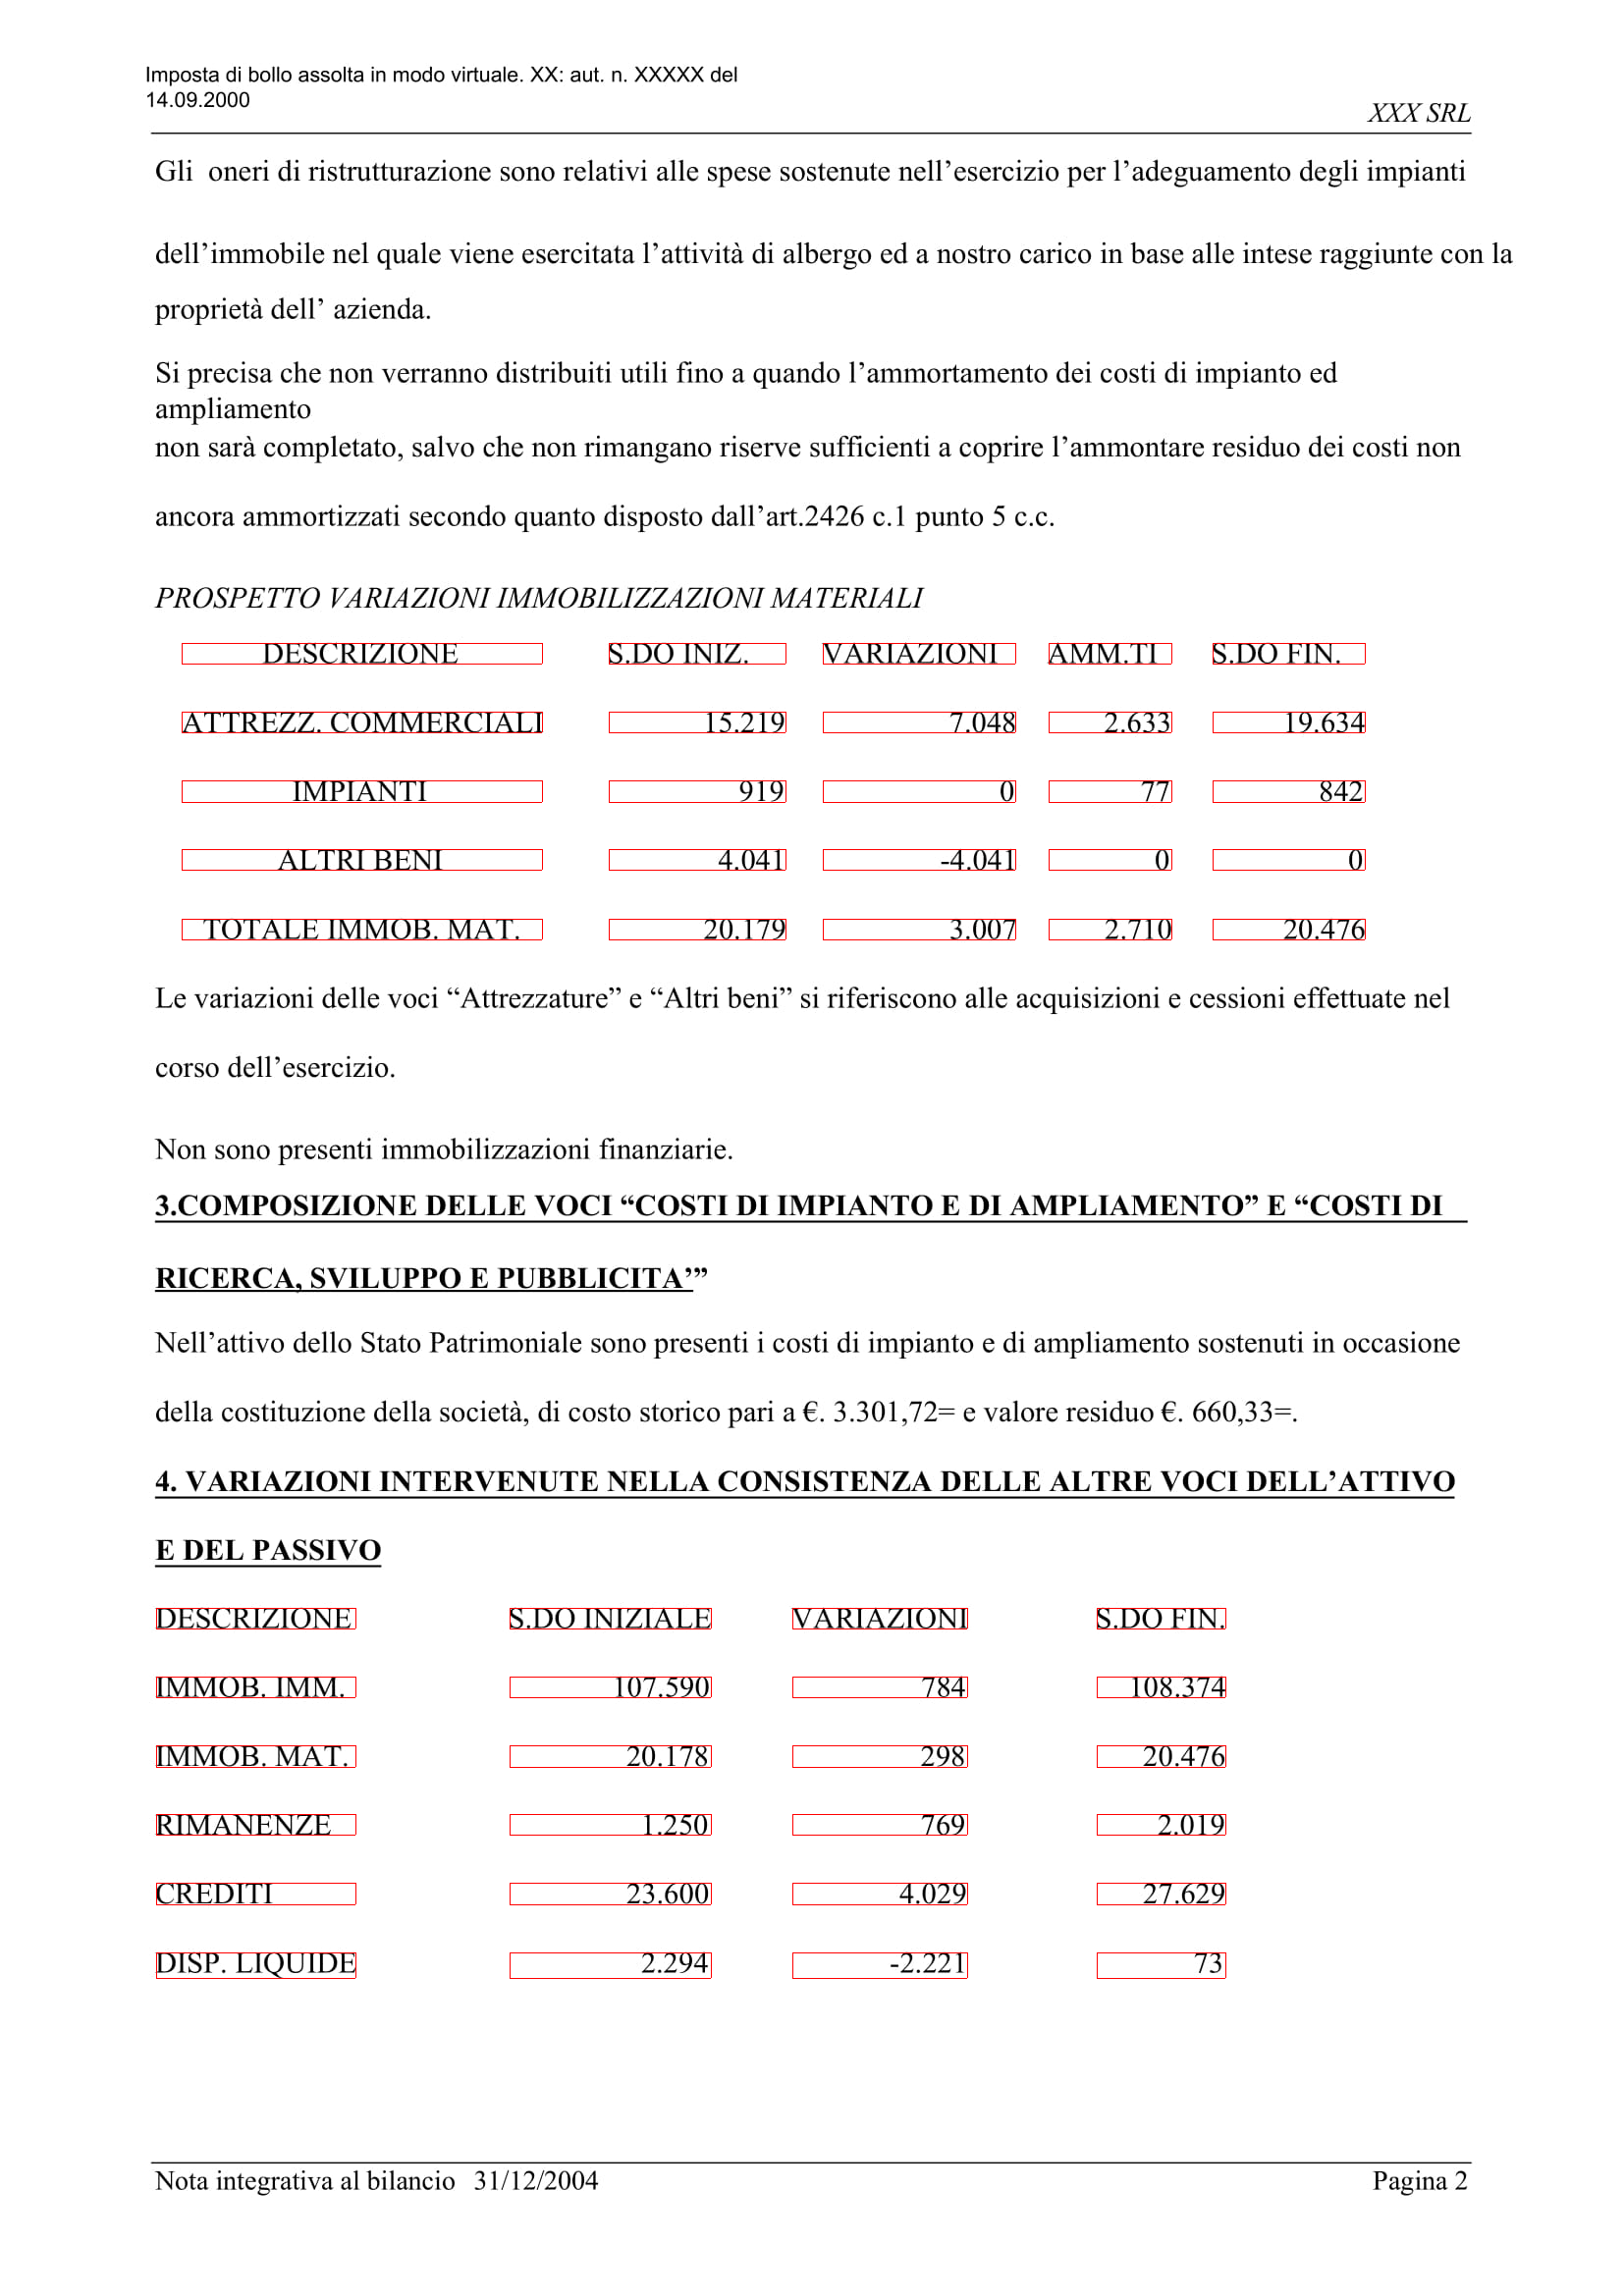
\includegraphics[width=15em]{img/results/goodRes2.png}
\caption{Correct recognition of tables \xxx{TO DO - nas algoritmus to tuto robi spravne}}
\label{fig:errors}
\end{figure}